% Szglab4
% ===========================================================================
%
\chapter{Analízis modell kidolgozása 1}

\thispagestyle{fancy}

\section{Objektum katalógus}

\subsection{Játékos}
Három vagy több van belőle. Körökre bontva teszik a dolgukat. Saját körükben tudnak mozogni, különböző tárgyakat használni vagy a speciális képességüket használni. A játék megnyeréséhez szükséges rakétapisztoly alkatrészek összegyűjétse a feladatuk. Ha vízbe esnek, vagy kihűlnek akkor a játéknak vége.

\subsection{Jégtábla}
Ilyenek alkotják a játékos számára a játékteret, ezeken lehet mozogni. Jégtáblák tartalmazhatnak tárgyakat amelyeket ki lehet ásni. Az instabil jégtábla képes vízbe ejteni a rajta állókat, ha túl sokan vannak. A jégtáblán lehet hó. Néha lehet rajta hóvihar, mely csökkenti a rajta állók testhőjét

\subsection{Kötél}
Ennek segítésével ki lehet húzni egy vízbe esett játékost.

\subsection{Búvárruha}
A jétékos képes a vízben is mozogni vele, illetve nem veszít testhőt ha vízben tartózkodik.

\subsection{Lapát}
Segítségével 2 egységnyi hó takarítható el a egy adott tábláról.

\subsection{Élelem}
Ha a játékos elfogyasztja a testhője 1-el megnő.

\subsection{Rakétapisztoly Alkatrész}
A játékban 3 darab ilyen megtalálása vezet a játék sikeres befejezéséhez. Az összeszereléshez mindháromnak egy helyen kell lennie.

\subsection{Iglu}
Eszkimó (Játékos) képes építeni, itt átvészelhetőek a hóviharok

\section{Statikus struktúra diagramok}
\comment{Az előző alfejezet osztályainak kapcsolatait és publikus metódusait bemutató osztálydiagram(ok). Tipikus hibalehetőségek: csillag-topológia, szigetek.}

\begin{figure}[h]
\begin{center}
%\includegraphics[width=17cm]{chapters/chapter03/example.pdf}
\caption{x}
\label{fig:example1}
\end{center}
\end{figure}


\section{Osztályok leírása}
\comment{Az előző alfejezetben tárgyalt objektumok felelősségének formalizálása attribútumokká, metódusokká. Csak publikus metódusok szerepelhetnek. Ebben az alfejezetben megjelennek az interfészek, az öröklés, az absztrakt osztályok. Segédosztályokra még mindig nincs szükség. Az osztályok ABC sorrendben kövessék egymást. Interfészek esetén az Interfészek, Attribútumok pontok kimaradnak.}

\subsection{BareHands}
\begin{itemize}
\item A játékos így ás, ha nincs ásója\\

\item Interfészek\\
DigStrategy

\item Metódusok
	\begin{itemize}
		\item bool Dig(Tile t): Csökkenti a tile-on található hó mennyiségét (int)
	\end{itemize}
\end{itemize}

\subsection{BareIce}
\begin{itemize}
\item A jégtáblán nincs védelem a vihar elől\\

\item Interfészek\\
ChillStormStrategy

\item Metódusok
	\begin{itemize}
		\item void Chill(Tile t): Táblán található játékos testhője csökken
	\end{itemize}
\end{itemize}

\subsection{CantRescue}
\begin{itemize}
	\item A játékos nemtudja kihúzni a csapattársát\\
	
\item Interfészek\\
RescueStrategy

\item Metódusok
\begin{itemize}
	\item void Rescue(Tile water, Tile land): üres
\end{itemize}
\end{itemize}

\subsection{ChillStormStrategy}
\begin{itemize}
	\item A Tile így hűti a viharban a játékosokat\\

	\item Metódusok
	\begin{itemize}
		\item abstract void Chill(Tile t)
	\end{itemize}
\end{itemize}

\subsection{ChillWaterStrategy}
\begin{itemize}
	\item  A Tile így hűti a vízbe esett játékosokat\\
	
\item Metódusok
\begin{itemize}
	\item abstract void Chill(Tile t)
\end{itemize}
\end{itemize}

\subsection{DigStrategy}
\begin{itemize}
	\item A játékos így ás\\
	
\item Metódusok
\begin{itemize}
	\item abstract bool Dig(Tile t)
\end{itemize}
\end{itemize}

\subsection{DryLand}
\begin{itemize}
	\item A szárazföld nem hűti a játékosokat\\
	
\item Interfészek\\
ChillWaterStrategy
\item Metódusok
\begin{itemize}
	\item void Chill(Tile t): üres
\end{itemize}
\end{itemize}

\subsection{Empty}
\begin{itemize}
	\item Nincs jégbe fagyott tárgy\\
	
\item Interfészek\\
GiveItemStrategy
\item Metódusok
\begin{itemize}
	\item void GiveTo(Player p): üres
\end{itemize}
\end{itemize}

\subsection{Eskimo}
\begin{itemize}
	\item Játékos típus, akivel valaki játszhat\\
	
	\item Ősosztályok\\
	Player
\item Metódusok
\begin{itemize}
	\item void BuildIgloo(): Épít egy iglut az adott mezőre
\end{itemize}
\end{itemize}

\subsection{Food}
\begin{itemize}
	\item Élelem amit a játékos meg tud enni, hogy növelje a testhőjét\\
	
\item Interfészek\\
GiveItemStrategy

\item Metódusok
\begin{itemize}
	\item void GiveTo(Player p): A játékos kap egy élelmet
\end{itemize}
\end{itemize}

\subsection{FoodStore}
\begin{itemize}
	\item A játékos ebben a zsebben tárolja az élelmet\\

\item Attribútumok\\

\begin{itemize}
	\item count: int: Hány élelem van a játékosnál

\end{itemize}
\item Metódusok\\
\begin{itemize}
	\item void feed(Player p): Játékos testhője megnő
\end{itemize}
\end{itemize}

\subsection{Game}
\begin{itemize}
	\item Interface a modell és a kontroller között. A játékmesterhez tartozó működést valósítja meg.\\
	
\item Attribútumok\\

\begin{itemize}
	\item players: Player[3..*]: Tárolja a játékosokat
	\item icefield: Tile[1..*]: Tárolja a pályát alkotó elemeket
\end{itemize}
\item Metódusok\\
\begin{itemize}
	\item Tile CreateIce(): Létrehoz egy jégtáblát. Ez a metódus az init szekvencia része.
	\item Tile CreateUnstableIce(): Létrehoz egy instabil jégtáblát. Ez a metódus az init szekvencia része.
	\item Tile CreateSea(): Létrehoz egy vizet. Ez a metódus az init szekvencia része.
	\item Tile CreateHole(): Létrehoz egy lyukat. Ez a metódus az init szekvencia része.
	\item Player CreateEskimo(): Létrehoz egy eszkimó játékost. Ez a metódus az init szekvencia része.
	\item Player CreatePolarExplorer(): Létrehoz egy sarkkutató játékost. Ez a metódus az init szekvencia része.
	\item void GameOver(): Ha vége a játéknak szól a Controllernek, hogy vesztettünk. Külső metódus
	\item void Turn(): Ezt a metódust a controller hívja. 
	\item void Victory(): Ha vége a játéknak szól a Controllernek, hogy nyertünk. Külső metódus
\end{itemize}
\end{itemize}

\subsection{Igloo}
\begin{itemize}
	\item Ezen a jégtáblán iglu áll, a játékosok védve vannak a vihartól\\
	
\item Interfészek\\
ChillStromStrategy
\item Metódusok
\begin{itemize}
	\item void Chill(Tile t): üres
\end{itemize}
\end{itemize}

\subsection{Naked}
\begin{itemize}
	\item A játékos védtelen a hideg vízzel szemben\\
	
\item Interfészek\\
WaterResistanceStrategy
\item Metódusok
\begin{itemize}
	\item void Chill(Player p): Játékosnak nincsen ereje a vízben úszni a ruha nélkül
\end{itemize}
\end{itemize}

\subsection{Part}
\begin{itemize}
	\item Jégbefagyott alkatrész\\

\item Interfészek\\
GiveItemStrategy

\item Metódusok\\
\begin{itemize}
	\item void GiveTo(Player p): A játékos tárolójába kerül egy darab a rakétapisztolyból
\end{itemize}
\end{itemize}

\subsection{PartStore}
\begin{itemize}
	\item A játékos ebben a zsebben tárolja az alkatrészeket\\
	
\item Attribútumok\\
\begin{itemize}
	\item count: int: Hány darab alkatrész van belőle a játékosnál
\end{itemize}
\item Metódusok\\
\begin{itemize}
	\item void Take(PartStore ps): Átveszi az alkatrészeket
	\item void Gain(int n): Megnő az alkatrészek száma ami a játékosnál van
	\item void Build(): Összerakja a rakétapisztolyt
\end{itemize}
\end{itemize}

\subsection{Player}
\begin{itemize}
	\item Játékos osztály, amit a játékos irányít a grafikus felületen keresztül\\

\item Attribútumok
\begin{itemize}
	\item bodyTemp: int: Jelzi a játékos jelenlegi hőmérsékletét, ha 0 akkor megfagy $\rightarrow$ játék vége
	\item currentTile: Tile: A játékos ismeri a mezőt amin éppen áll
	\item digStrategy: DigStrategy: Eldönti hogyan képes ásni a játékos
	\item energy: int: Számlálja mennyit mozogott az adott körben a játékos
	\item foodStore: FoodStore: Tárolja a játékos ételeit
	\item partStore: PartStore: Tárolja a játékos rakéta alkatrészeit
	\item rescueStrategy: RescueStrategy: Eldönti, hogy megmenthet egy játékos egy másikat a vízbeesés után
	\item waterResistanceStrategy: WaterResistanceStrategy: Eldönti, hogy a játékos hogy viselkedik vízbeesés esetén
\end{itemize}
\item Metódusok
\begin{itemize}
	\item void AssembleFlare(): Összerakja a játék végéhez szükséges rakéta pisztolyt.
	\item void Chill(): A testhő 1-el csökken, ha 0 alá megy GameOver.
	\item void Dig(): Ezt a metódust a controller hívja. A játékos havat ás.
	\item void EatFood(): Ezt a metódust a controller hívja. A játékos eszik.
	\item void PickUp(): Ezt a metódust a controller hívja. A játékos felvesz egy tárgyat.
	\item void PlaceOn(Tile t): Init szekvencia része. RopeRescue szekvencia része. Rárak egy játékost egy másik Tile-ra.
	\item void RescueTeammate(direction d): Ezt a metódust a controller hívja. A játékos kiment egy másikat a vízből.
	\item void ResistWater(): A játékos testhője a WaterResistance szerint változik.
	\item void Step(): Ezt a metódust a controller hívja. A játékos lép, ha van még hozzá elég energiája.
\end{itemize}
\end{itemize}


\subsection{PolarExplorer}
\begin{itemize}
	\item Játékos típus, akivel valaki játszhat\\
	
	\item Ősosztályok\\
	Player
\item Metódusok
\begin{itemize}
	\item void Examine(direction d): A játékos megnézheti, hogy egy adott Tile-nak mennyi a teherbírása
\end{itemize}
\end{itemize}

\subsection{RescueStrategy}
\begin{itemize}
	\item A játékos így húzza ki csapattársát a vízből.\\

\item Metódusok
\begin{itemize}
	\item abstract void Rescue(Tile water, Tile land): üres
\end{itemize}
\end{itemize}

\subsection{Rope}
\begin{itemize}
	\item Jégbe fagyott kötél\\
\item Interfészek\\
GiveItemStrategy
\item Metódusok
\begin{itemize}
	\item void GiveTo(Player p): Felrhuázza a játékos a megmentésre alkalmas eszközzel.
\end{itemize}
\end{itemize}

\subsection{RopeRescue}
\begin{itemize}
	\item A játékos kihúzza csapattársát a vízből.\\
\item Interfészek\\
RescueStrategy

\item Metódusok
\begin{itemize}
	\item void Rescue(Tile water, Tile land): A játékos kihúzza a vízbe esett csapattárását a vízből, ha van kötele.
\end{itemize}
\end{itemize}

\subsection{ScubaGear}
\begin{itemize}
	\item Jégbe fagyott búvárruha.\\
\item Interfészek\\
GiveItemStrategy
\item Metódusok\\
\begin{itemize}
	\item void GiveTo(): Felrhuázza a játékos a vízben maradásra alkalmas eszközzel.
\end{itemize}
\end{itemize}

\subsection{Sea}
\begin{itemize}
	\item Ez a cella tenger, hűti a játékosokat.\\
\item Interfészek\\
ChillWaterStrategy

\item Metódusok
\begin{itemize}
	\item void Chill(Tile t): Minden rajta álló testhője csökken a WaterResistanceStrategy szerint.
\end{itemize}
\end{itemize}

\subsection{ShovelDig}
\begin{itemize}
	\item Egyszer lehet ásni vele fáradság nélkül is\\
\item Interfészek\\
DigStrategy

\item Attribútumok
\begin{itemize}
	\item lastUsed: bool: Volt e már használva a körben
\end{itemize}
\item Metódusok
\begin{itemize}
	\item void Dig(Tile t): Csökkenti a tile-on található hó mennyiségét (int)
\end{itemize}
\end{itemize}

\subsection{Tile}
\begin{itemize}
	\item Ilyenekből áll a jégmező ahol a játékosok játszanak.\\
\item Attribútumok
\begin{itemize}
	\item chillStormStrategy: ChillStormStrategy:Eldönti kinek változik a testhője vihar esetén.
	\item chillWaterStrategy: ChillWaterStrategy: Eldönti kinek változik a testhője víz esetén.
	\item giveItemStrategy: GiveItemStrategy: Eldönti milyen eszközt vett fel valaki.
	\item neighborTiles: Tile[*]: Szomszédos cellákat tárolja, ismeri.
	\item occupants: Player[*]: Rajta lévő játékosok.
	\item snow: int: Rajta lévő hómennyiség
	\item weightLimit: int: Rajta lévő játékosok számának maximuma.
	
\end{itemize}
\item Metódusok
\begin{itemize}
	\item void AddOccupant(Player p): Rátesz egy játékost a cellára.
	\item void RemoveOccupant(Player p): Levesz egy játékos a celláról.
	\item void ChillStorm(): Ezt a metódust a Controller hívja. Hűti a játékosokat.
	\item void GiveItem(Player): A játékos megkapja a felvett tárgyat.
	\item Tile NeighborAt(direction): Visszaadja az adott irányba lévő cellát.
	\item StepOn(Player):
	\item StepOff(Player):
\end{itemize}
\end{itemize}

\subsection{WaterResistanceStrategy}
\begin{itemize}
	\item Így reagál a játékos a hideg vízre.\\
\item Metódusok
\begin{itemize}
	\item abstract void Chill(Player p): üres
\end{itemize}
\end{itemize}

\section{Statikus struktúra diagramok}
\comment{Az előző alfejezet osztályainak kapcsolatait és publikus metódusait bemutató osztálydiagram(ok). Tipikus hibalehetőségek: csillag-topológia, szigetek.}

%\begin{figure}[h]
%\begin{center}
%\includegraphics[width=17cm]{chapters/chapter03/example.pdf}
%\caption{x}
%\label{fig:example1}
%\end{center}
%\end{figure}
\newpage
\section{Szekvencia diagramok}
%\comment{Inicializálásra, use-case-ekre, belső működésre. Konzisztens kell legyen az előző alfejezettel. Minden metódus, ami ott szerepel, fel kell tűnjön valamelyik szekvenciában. Minden metódusnak, ami szekvenciában szerepel, szereplnie kell a valamelyik osztálydiagramon.}
%find . -printf "\\\begin{figure}[H]\n\t\\\begin{center}\n\t\t\\\includegraphics[width=10cm]{chapters/chapter03/seqdiag/%f}\n\t\t\\\caption{aaa}\n\t\t\\\label{bbb}\n\t\\\end{center}\n\\\end{figure}\n"
\begin{figure}[H]
	\begin{center}
		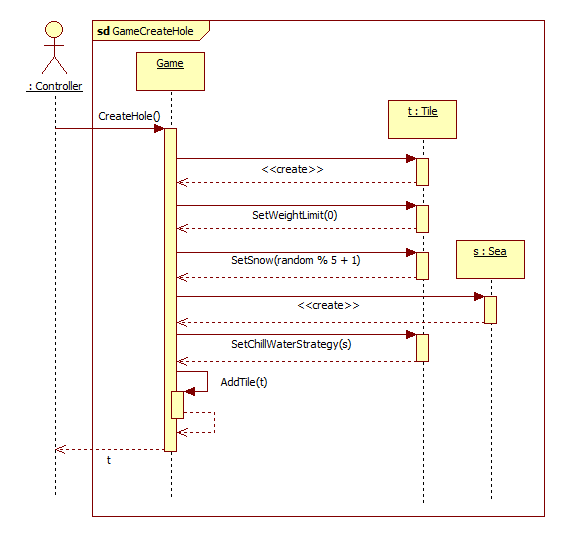
\includegraphics[width=10cm]{chapters/chapter03/seqdiag/Game_CreateHole.png}
		\caption{Game.CreateHole()}
		\label{fig:GameCreateHole}
	\end{center}
\end{figure}
\begin{figure}[H]
	\begin{center}
		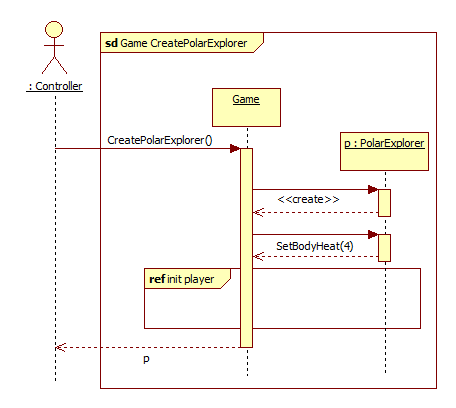
\includegraphics[width=10cm]{chapters/chapter03/seqdiag/Game_CreatePolarExplorer.png}
		\caption{Game.CreatePolarExplorer()}
		\label{fig:GameCreatePolarExplorer}
	\end{center}
\end{figure}
\begin{figure}[H]
	\begin{center}
		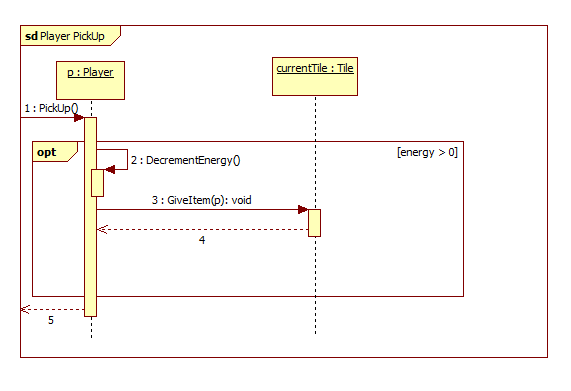
\includegraphics[width=10cm]{chapters/chapter03/seqdiag/Player_PickUp.png}
		\caption{Player.PickUp()}
		\label{fig:PlayerPickUp}
	\end{center}
\end{figure}
\begin{figure}[H]
	\begin{center}
		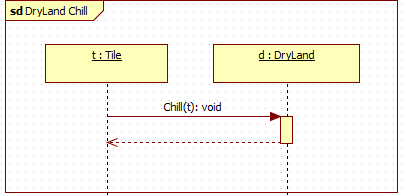
\includegraphics[width=10cm]{chapters/chapter03/seqdiag/DryLand_Chill.png}
		\caption{DryLand.Chill(Tile)}
		\label{fig:DryLandChill}
	\end{center}
\end{figure}
\begin{figure}[H]
	\begin{center}
		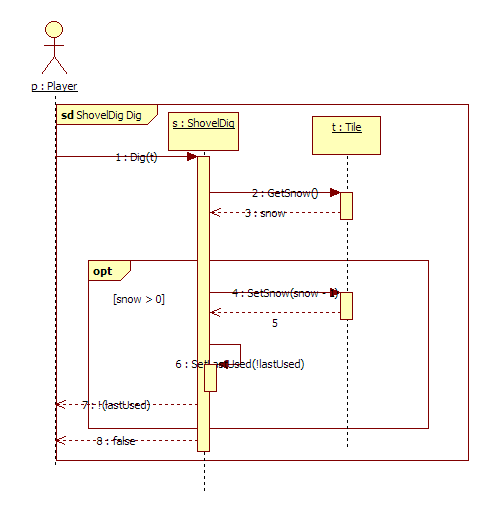
\includegraphics[width=10cm]{chapters/chapter03/seqdiag/ShovelDig_Dig.png}
		\caption{ShovelDig.Dig(Tile)}
		\label{fig:ShovelDigDig}
	\end{center}
\end{figure}
\begin{figure}[H]
	\begin{center}
		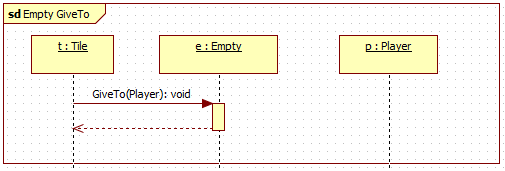
\includegraphics[width=10cm]{chapters/chapter03/seqdiag/Empty_GiveTo.png}
		\caption{Empty.GiveTo(Player)}
		\label{fig:EmptyGiveTo}
	\end{center}
\end{figure}
\begin{figure}[H]
	\begin{center}
		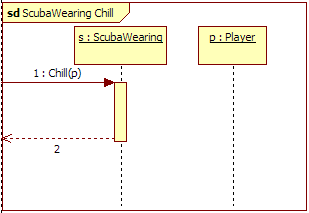
\includegraphics[width=10cm]{chapters/chapter03/seqdiag/ScubaWearing_Chill.png}
		\caption{ScubaWearing.Chill(Player)}
		\label{fig:ScubaWearingChill}
	\end{center}
\end{figure}
\begin{figure}[H]
	\begin{center}
		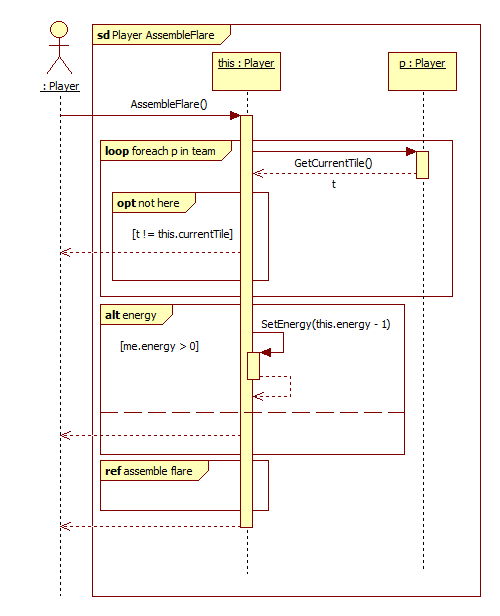
\includegraphics[width=10cm]{chapters/chapter03/seqdiag/Player_AssembleFlare.png}
		\caption{Player.AssembleFlare()}
		\label{fig:PlayerAssembleFlare}
	\end{center}
\end{figure}
\begin{figure}[H]
	\begin{center}
		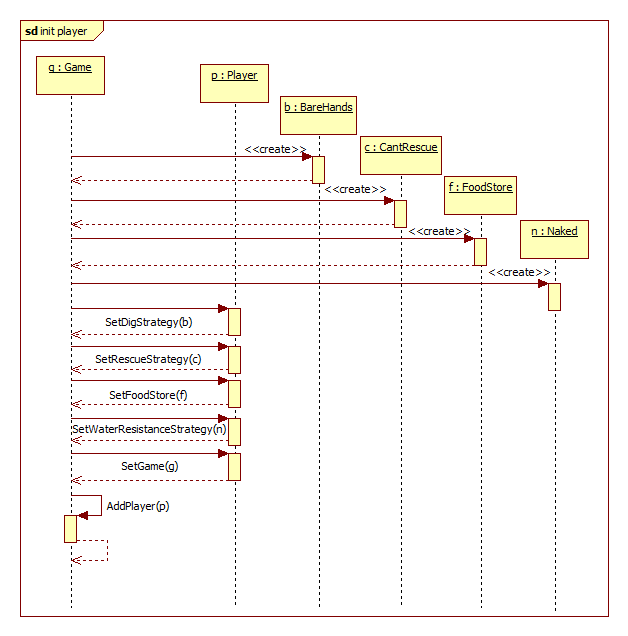
\includegraphics[width=10cm]{chapters/chapter03/seqdiag/Game_init_player.png}
		\caption{Game.InitPlayer()}
		\label{fig:GameInitPlayer}
	\end{center}
\end{figure}
\begin{figure}[H]
	\begin{center}
		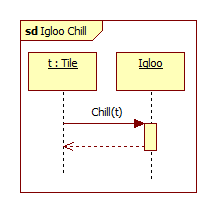
\includegraphics[width=10cm]{chapters/chapter03/seqdiag/Igloo_Chill.png}
		\caption{Igloo.Chill(Tile)}
		\label{fig:IglooChill}
	\end{center}
\end{figure}
\begin{figure}[H]
	\begin{center}
		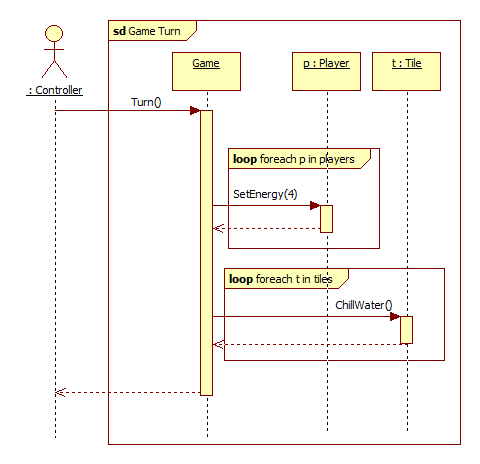
\includegraphics[width=10cm]{chapters/chapter03/seqdiag/Game_Turn.png}
		\caption{Game.Turn()}
		\label{fig:GameTurn}
	\end{center}
\end{figure}
\begin{figure}[H]
	\begin{center}
		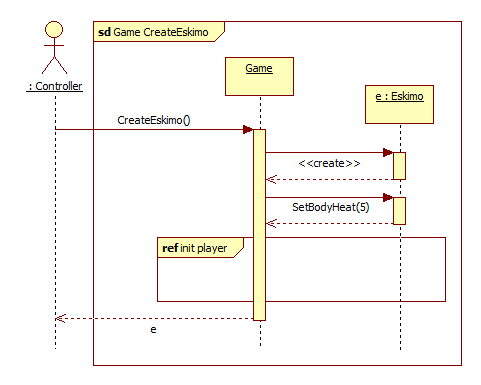
\includegraphics[width=10cm]{chapters/chapter03/seqdiag/Game_CreateEskimo.png}
		\caption{Game.CreateEskimo()}
		\label{fig:GameCreateEskimo}
	\end{center}
\end{figure}
\begin{figure}[H]
	\begin{center}
		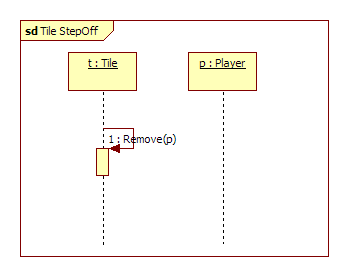
\includegraphics[width=10cm]{chapters/chapter03/seqdiag/Tile_StepOff.png}
		\caption{Tile.StepOff(Player)}
		\label{fig:TileStepOff}
	\end{center}
\end{figure}
\begin{figure}[H]
	\begin{center}
		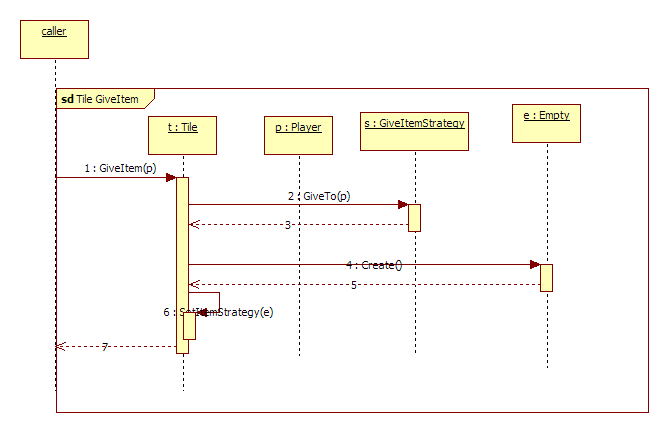
\includegraphics[width=10cm]{chapters/chapter03/seqdiag/Tile_GiveItem.png}
		\caption{Tile.GiveItem(Player)}
		\label{fig:TileGiveItem}
	\end{center}
\end{figure}
\begin{figure}[H]
	\begin{center}
		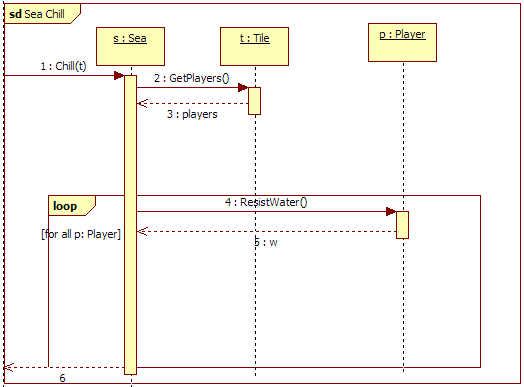
\includegraphics[width=10cm]{chapters/chapter03/seqdiag/Sea_Chill.png}
		\caption{Sea.Chill(Tile)}
		\label{fig:SeaChill}
	\end{center}
\end{figure}
\begin{figure}[H]
	\begin{center}
		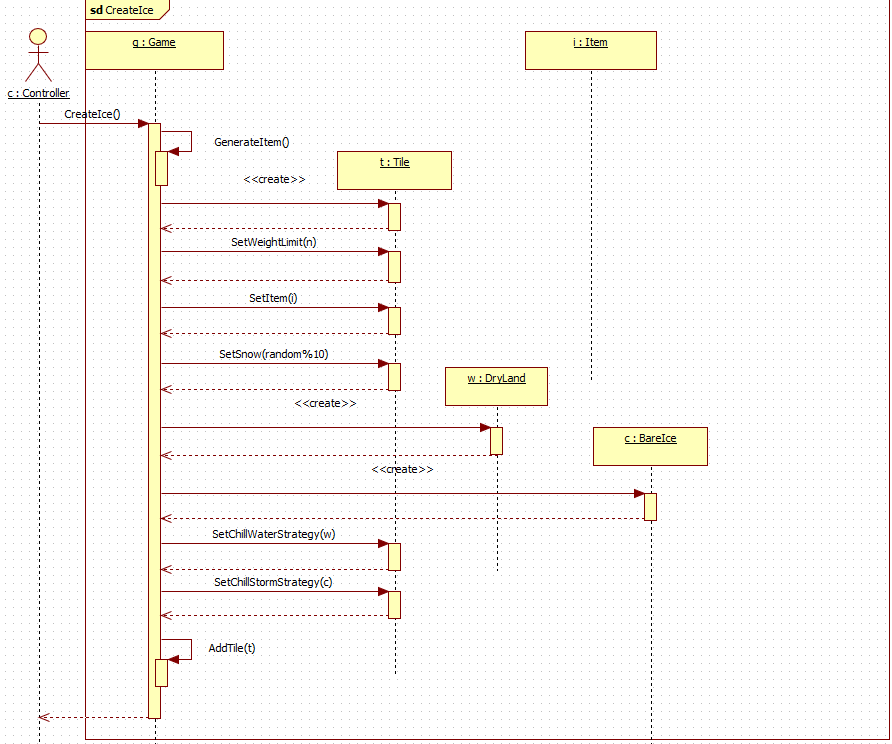
\includegraphics[width=10cm]{chapters/chapter03/seqdiag/Game_CreateIce.png}
		\caption{Game.CreateIce()}
		\label{fig:GameCreateIce}
	\end{center}
\end{figure}
\begin{figure}[H]
	\begin{center}
		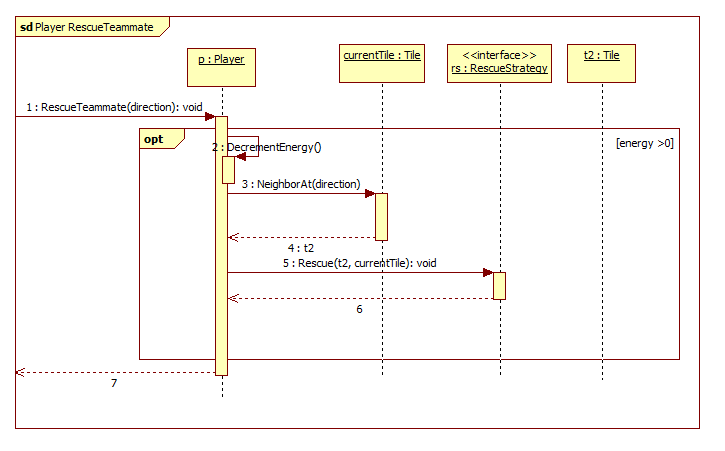
\includegraphics[width=10cm]{chapters/chapter03/seqdiag/Player_RescueTeammate.png}
		\caption{Player.RescueTeammate(direction)}
		\label{fig:Player.RescueTeammate}
	\end{center}
\end{figure}
\begin{figure}[H]
	\begin{center}
		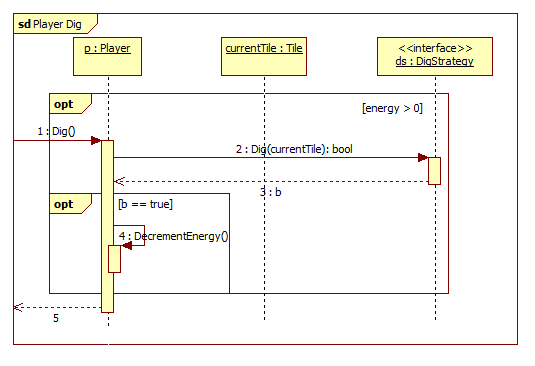
\includegraphics[width=10cm]{chapters/chapter03/seqdiag/Player_Dig.png}
		\caption{Player.Dig()}
		\label{fig:PlayerDig}
	\end{center}
\end{figure}
\begin{figure}[H]
	\begin{center}
		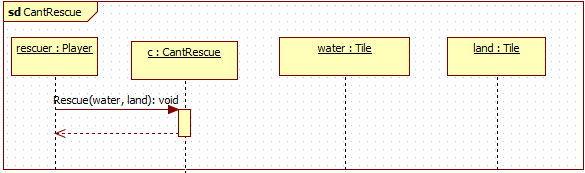
\includegraphics[width=10cm]{chapters/chapter03/seqdiag/CantRescue_Rescue.png}
		\caption{CantRescue.Rescue(Tile, Tile)}
		\label{fig:CantRescueRescue}
	\end{center}
\end{figure}
\begin{figure}[H]
	\begin{center}
		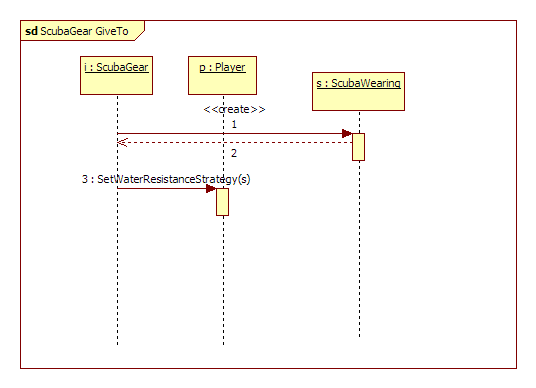
\includegraphics[width=10cm]{chapters/chapter03/seqdiag/ScubaGear_GiveTo.png}
		\caption{ScubaGear.GiveTo(Player)}
		\label{fig:ScubaGearGiveTo}
	\end{center}
\end{figure}
\begin{figure}[H]
	\begin{center}
		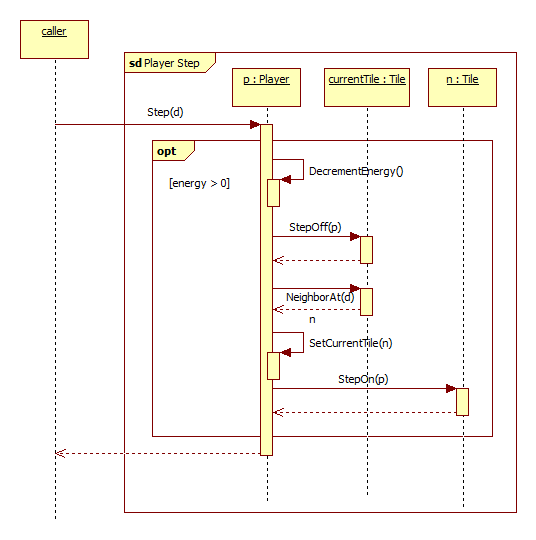
\includegraphics[width=10cm]{chapters/chapter03/seqdiag/Player_Step.png}
		\caption{Player.Step(direction)}
		\label{fig:PlayerStep}
	\end{center}
\end{figure}
\begin{figure}[H]
	\begin{center}
		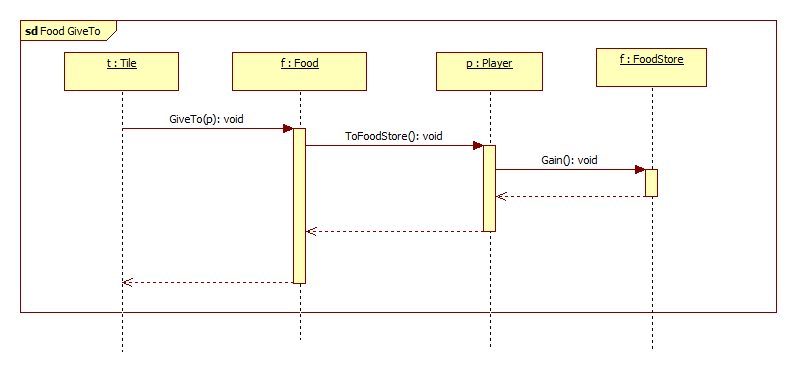
\includegraphics[width=10cm]{chapters/chapter03/seqdiag/Food_GiveTo.png}
		\caption{Food.GiveTo(Player)}
		\label{fig:FoodGiveTo}
	\end{center}
\end{figure}
\begin{figure}[H]
	\begin{center}
		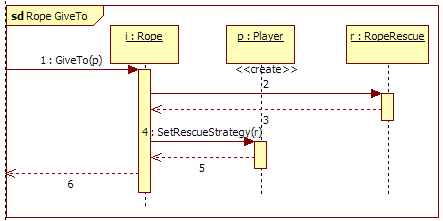
\includegraphics[width=10cm]{chapters/chapter03/seqdiag/Rope_GiveTo.png}
		\caption{Rope.GiveTo(Player)}
		\label{fig:RopeGiveTo}
	\end{center}
\end{figure}
\begin{figure}[H]
	\begin{center}
		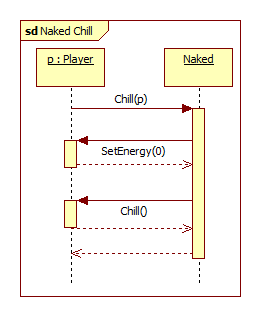
\includegraphics[width=10cm]{chapters/chapter03/seqdiag/Naked_Chill.png}
		\caption{Naked.Chill(Player)}
		\label{fig:NakedChill}
	\end{center}
\end{figure}
\begin{figure}[H]
	\begin{center}
		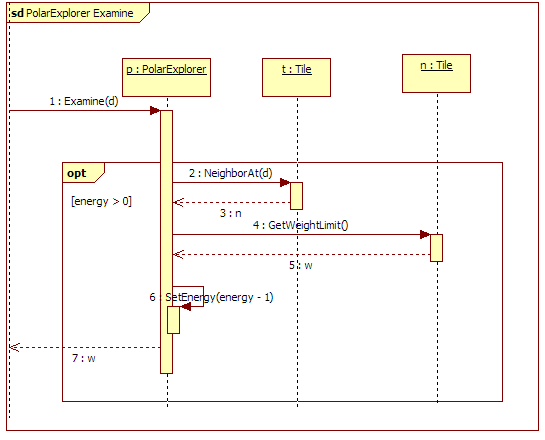
\includegraphics[width=10cm]{chapters/chapter03/seqdiag/PolarExplorer_Examine.png}
		\caption{PolarExplorer.Examine(direction)}
		\label{fig:PolarExplorerExamine}
	\end{center}
\end{figure}
\begin{figure}[H]
	\begin{center}
		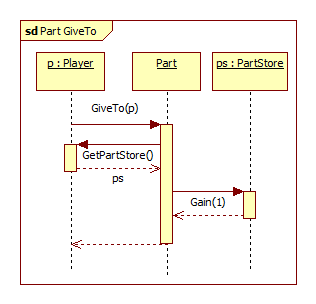
\includegraphics[width=10cm]{chapters/chapter03/seqdiag/Part_GiveTo.png}
		\caption{Part.GiveTo(Player)}
		\label{fig:PartGiveTo}
	\end{center}
\end{figure}
\begin{figure}[H]
	\begin{center}
		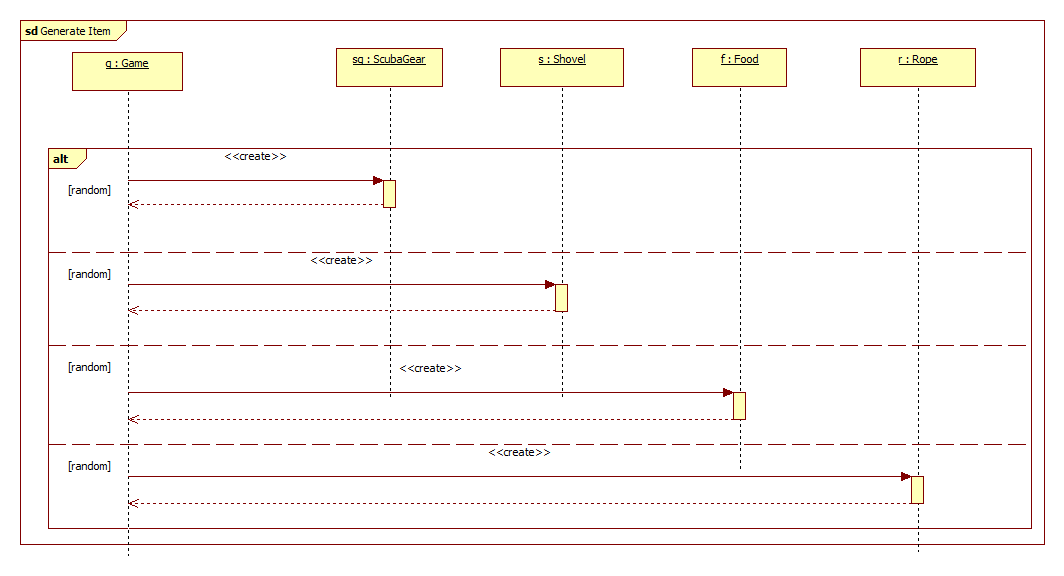
\includegraphics[width=10cm]{chapters/chapter03/seqdiag/Game_generate_item.png}
		\caption{Game.GenerateItem()}
		\label{fig:GameGenerateItem}
	\end{center}
\end{figure}
\begin{figure}[H]
	\begin{center}
		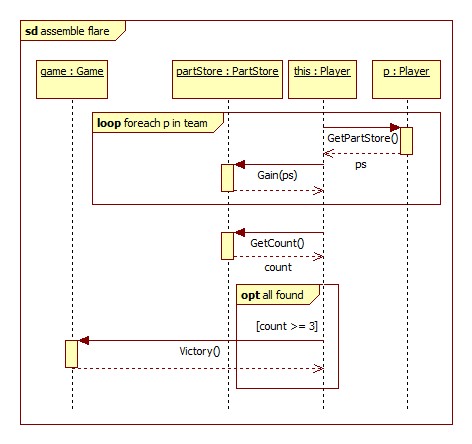
\includegraphics[width=10cm]{chapters/chapter03/seqdiag/Player_assemble_flare.png}
		\caption{Player.AssembleFlare()}
		\label{fig:PlayerAssembleFlare}
	\end{center}
\end{figure}
\begin{figure}[H]
	\begin{center}
		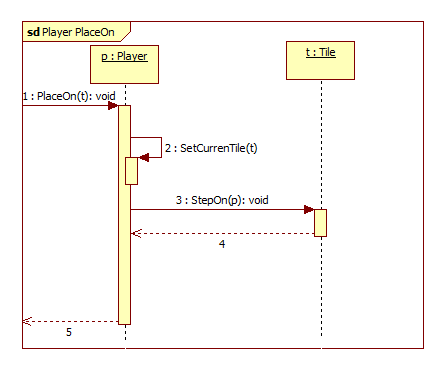
\includegraphics[width=10cm]{chapters/chapter03/seqdiag/Player_PlaceOn.png}
		\caption{Player.PlaceOn(Tile)}
		\label{fig:PlayerPlaceOn}
	\end{center}
\end{figure}
\begin{figure}[H]
	\begin{center}
		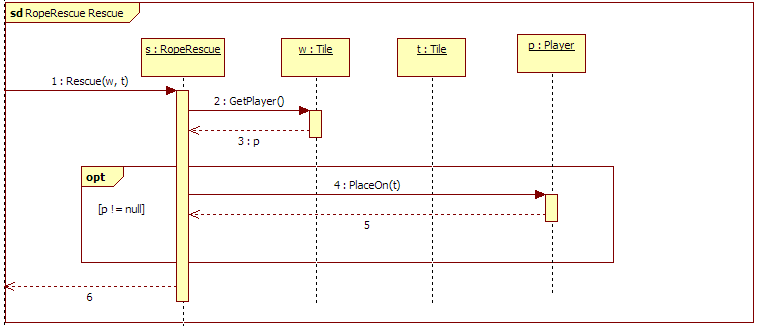
\includegraphics[width=10cm]{chapters/chapter03/seqdiag/RopeRescue_Rescue.png}
		\caption{RopeRescue.Rescue(Tile, Tile)}
		\label{fig:RopeRescueRescue}
	\end{center}
\end{figure}
\begin{figure}[H]
	\begin{center}
		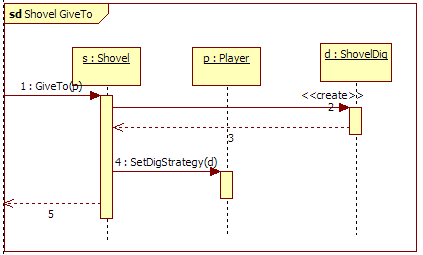
\includegraphics[width=10cm]{chapters/chapter03/seqdiag/Shovel_GiveTo.png}
		\caption{Shovel.GiveTo(Player)}
		\label{fig:ShovelGiveTo}
	\end{center}
\end{figure}
\begin{figure}[H]
	\begin{center}
		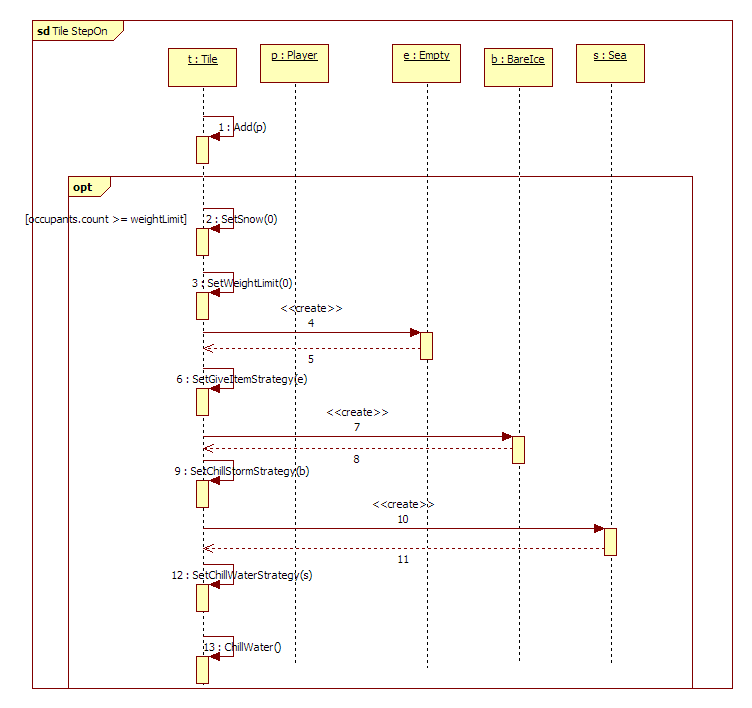
\includegraphics[width=10cm]{chapters/chapter03/seqdiag/Tile_StepOn.png}
		\caption{Tile.StepOn(Player)}
		\label{fig:TileStepOn}
	\end{center}
\end{figure}
\begin{figure}[H]
	\begin{center}
		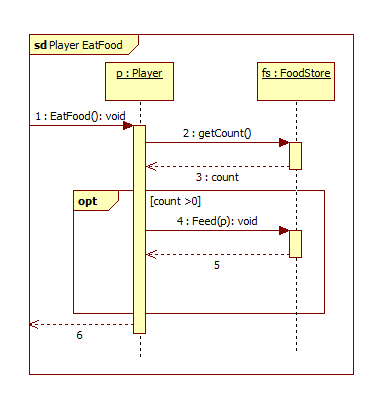
\includegraphics[width=10cm]{chapters/chapter03/seqdiag/Player_EatFood.png}
		\caption{Player.EatFood()}
		\label{fig:PlayerEatFood}
	\end{center}
\end{figure}
\begin{figure}[H]
	\begin{center}
		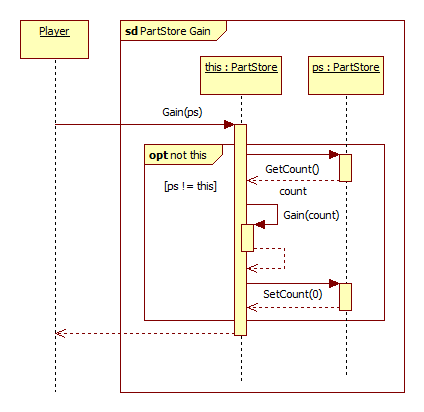
\includegraphics[width=10cm]{chapters/chapter03/seqdiag/PartStore_Gain.png}
		\caption{PartStore.Gain(PartStore)}
		\label{fig:PartStoreGain}
	\end{center}
\end{figure}
\begin{figure}[H]
	\begin{center}
		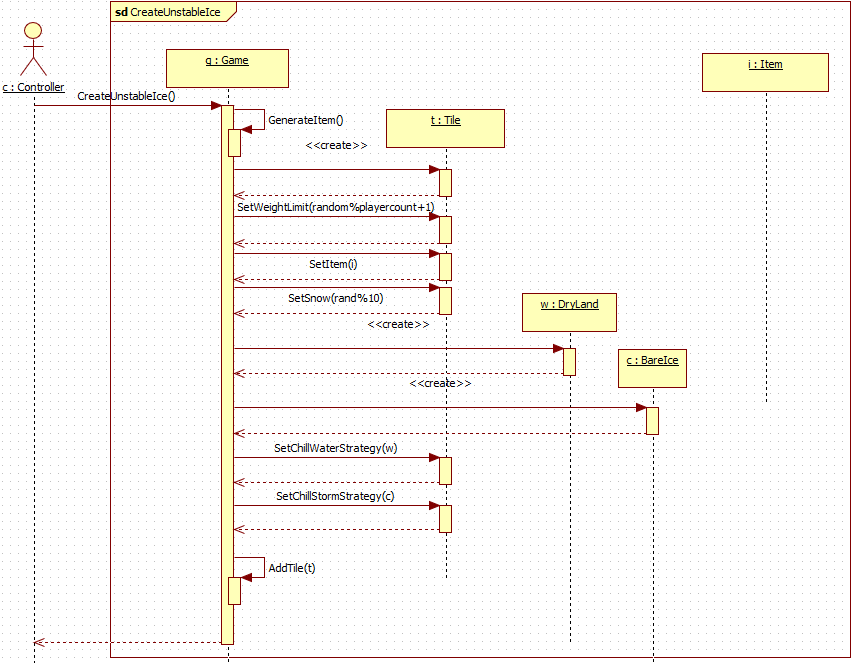
\includegraphics[width=10cm]{chapters/chapter03/seqdiag/Game_CreateUnstableIce.png}
		\caption{Game.CreateUnstableIce()}
		\label{fig:GameCreateUnstableIce}
	\end{center}
\end{figure}
\begin{figure}[H]
	\begin{center}
		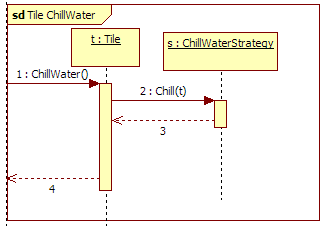
\includegraphics[width=10cm]{chapters/chapter03/seqdiag/Tile_ChillWater.png}
		\caption{Tile.ChillWater()}
		\label{fig:TileChillWater}
	\end{center}
\end{figure}
\begin{figure}[H]
	\begin{center}
		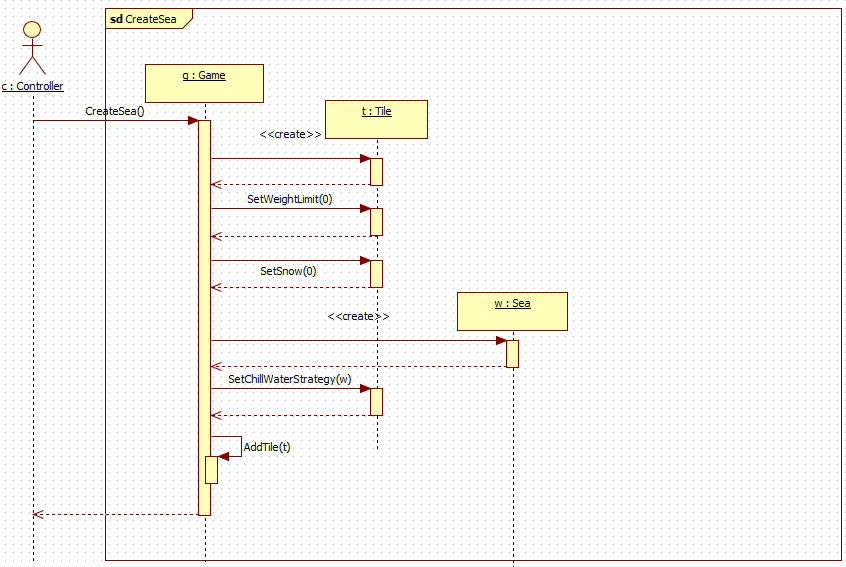
\includegraphics[width=10cm]{chapters/chapter03/seqdiag/Game_CreateSea.png}
		\caption{Game.CreateSea()}
		\label{fig:GameCreateSea}
	\end{center}
\end{figure}
\begin{figure}[H]
	\begin{center}
		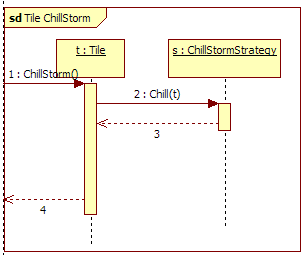
\includegraphics[width=10cm]{chapters/chapter03/seqdiag/Tile_ChillStorm.png}
		\caption{Tile.ChillStorm()}
		\label{fig:TileChillStorm}
	\end{center}
\end{figure}
\begin{figure}[H]
	\begin{center}
		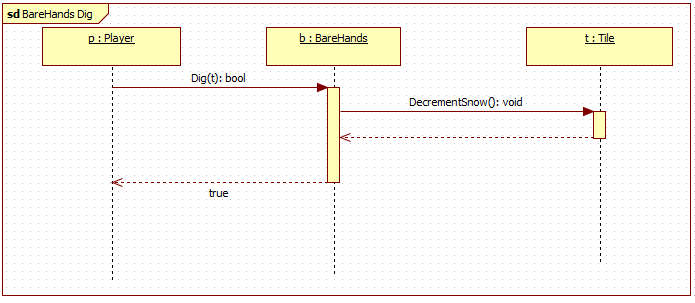
\includegraphics[width=10cm]{chapters/chapter03/seqdiag/BareHandsDig_Dig.png}
		\caption{BareHandsDig.Dig(Tile)}
		\label{fig:BareHandsDig.Dig}
	\end{center}
\end{figure}
\begin{figure}[H]
	\begin{center}
		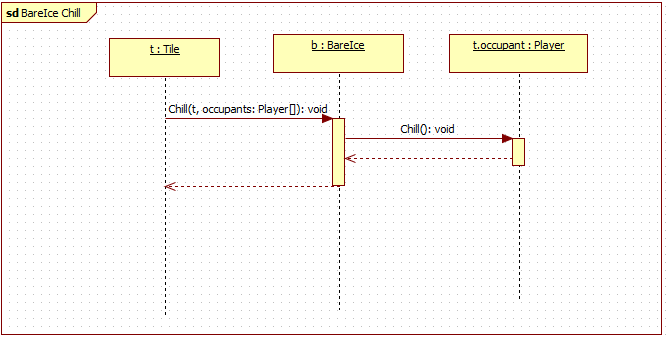
\includegraphics[width=10cm]{chapters/chapter03/seqdiag/BareIce_Chill.png}
		\caption{BareIce.Chill()}
		\label{fig:BareIceChill}
	\end{center}
\end{figure}
\begin{figure}[H]
	\begin{center}
		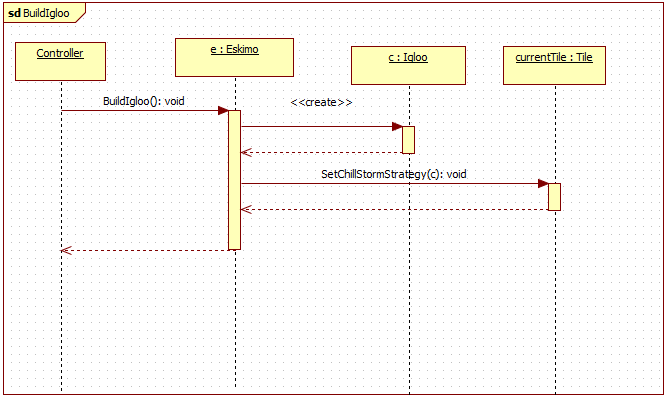
\includegraphics[width=10cm]{chapters/chapter03/seqdiag/Eskimo_BuildIgloo.png}
		\caption{Eskimo.BuildIgloo()}
		\label{fig:EskimoBuildIgloo}
	\end{center}
\end{figure}
\begin{figure}[H]
	\begin{center}
		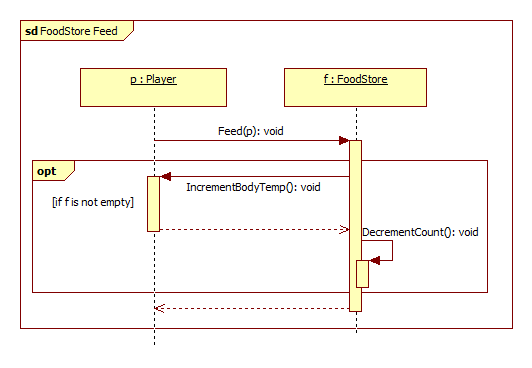
\includegraphics[width=10cm]{chapters/chapter03/seqdiag/FoodStore_Feed.png}
		\caption{FoodStore.Feed(Player)}
		\label{fig:FoodStoreFeed}
	\end{center}
\end{figure}
\begin{figure}[H]
	\begin{center}
		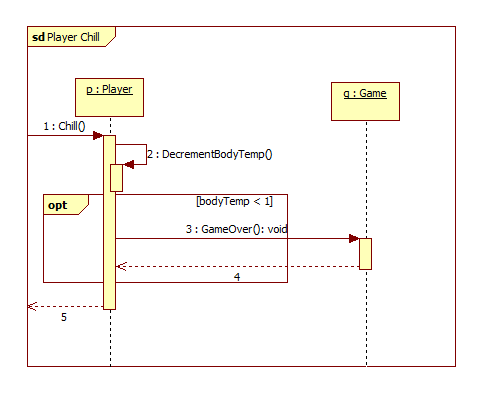
\includegraphics[width=10cm]{chapters/chapter03/seqdiag/Player_Chill.png}
		\caption{Player.Chill()}
		\label{fig:PlayerChill}
	\end{center}
\end{figure}
\begin{figure}[H]
	\begin{center}
		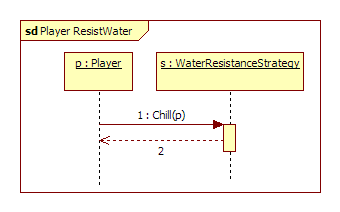
\includegraphics[width=10cm]{chapters/chapter03/seqdiag/Player_ResistWater.png}
		\caption{Player.ResistWater()}
		\label{fig:PlayerResistWater}
	\end{center}
\end{figure}



\section{State-chartok}
\comment{Csak azokhoz az osztályokhoz, ahol van értelme. Egyetlen állapotból álló state-chartok ne szerepeljenek. A játék működését bemutató state-chart-ot készíteni tilos.}
\newpage
%\begin{figure}[h]
%\begin{center}
%\includegraphics[width=17cm]{chapters/chapter03/example.pdf}
%\caption{x}
%\label{fig:example3}
%\end{center}
%\end{figure}

